\documentclass[a4paper,10pt]{article}

\usepackage[activeacute]{babel}
\usepackage[utf8]{inputenc}
\usepackage{bookman}
\usepackage{color}
\usepackage{graphicx}
\usepackage{anysize}
\usepackage{multicol}
\usepackage[pdftex=true,colorlinks=true,linkcolor=black,urlcolor=blue]{hyperref}

\marginsize{1.5cm}{1.5cm}{1.5cm}{1.5cm}
\newcommand{\HRule}{\rule{\linewidth}{0.5mm}}

\date{}

\pagenumbering{arabic}
\setcounter{page}{1}

\begin{document}

% ===================================== MEMBRETE ===================================== %
\begin{center}
  \textsc {
    Universidad Simón Bolívar \\[0cm]
    Departamento de Computaci\'on y Tecnolog\'ia de la Informaci\'on \\[0cm]
    CI5438 - Inteligencia Artificial I \\[0cm]
    Trimestre Abril - Julio 2021 \\[0cm]
    Prof. Carlos Infante \\[0cm]
    Amin Arriaga 16-10072, David Segura 13-11341, Wilfredo Graterol 15-10639
  }
  \HRule \\[0.4cm]
  {\Large \textbf{\'Arboles de juego}} \\[0.4cm]
  \textsc{
    \today
  }
  \HRule
\end{center}

\section*{othello\_t}
  Tomando como base la implementaci\'on incompleta de la clase \verb|state_t| del 
  profesor Blai Bonet, la cual renombramos como \verb|othello_t|, realizamos los 
  siguientes cambios que consideramos convenientes\footnote{En el repositorio se
  encuentra documentado todos los cambios realizados, as\'i como la explicaci\'on 
  de la implementaci\'on original. En esta secci\'on solo realizaremos un resumen 
  de las modificaciones.}:

  \begin{itemize}
    \item Se cre\'o una m\'etodo \verb|valid_moves| que, dado un color, retorna 
    un vector con las posibles jugadas de dicho color en el estado actual. Si no 
    se consigue ning\'un movimiento v\'alido, retorna el vector \verb|{36}|,  
    indicando que la \'unica jugada v\'alida es pasar. No se verifica si el estado 
    es terminal pues esa verificaci\'on se realiza en los algoritmos antes de 
    llamar a esta funci\'on, por lo que, para no realizar c\'alculos innecesarios,
    se hace la suposici\'on de que el estado no es terminal.

    \item Se modific\'o la funci\'on \verb|print| para que imprimiera una 
    representaci\'on del tablero mucho m\'as agradable. Sin embargo, debe ejecutarse 
    en una terminal que soporte los caracteres especiales de BASH para darle estilo
    al output. Tambi\'en se cre\'o una funci\'on \verb|print_board| que imprime 
    pr\'acticamente lo mismo, pero enumerando las filas y columnas.

    \item Se agregaron las verificaciones sobre las diagonales en las funciones 
    \verb|outflank| y \verb|move|, siendo pr\'acticamente iguales a las verificaciones
    de filas y columnas pero usando los vectores \verb|dia1| y \verb|dia2| en lugar 
    de \verb|rows| y \verb|cols|.
  \end{itemize}

\section*{Algoritmos}
  Las funciones \verb|negamax| (con y sin poda alpha-beta) y \verb|scout| fueron 
  implementados gui\'andonos por el pseudoc\'odigo visto en clases, mientras que 
  \verb|negascout| fue implementado gui\'andonos por la siguiente 
  \href{https://es.wikipedia.org/wiki/Negascout}{p\'agina} de Wikipedia, ya que el 
  de las l\'aminas ten\'ia un error que fue corregido luego de finalizar nuestra 
  implementaci\'on\footnote{Sin embargo, posteriormente se comprob\'o que el rendimiento del
  algoritmo que aparece en Wikipedia y el de las clases son iguales.}. La \'unica 
  diferencia con los pesudoc\'odigos y nuestras implementaciones es que en lugar 
  de iterar sobre los sucesores de un estado, se itera sobre sus posibles movimientos,
  usando la funci\'on \verb|valid_moves|, y en cada iteraci\'on se calcula el nuevo 
  estado sucesor. Esto es un poco m\'as eficiente en memoria pues no se mantienen 
  almacenados todos los sucesores de un estado en cada llamada recursiva.\\
  
  Cada algoritmo tiene su an\'alogo \verb|best_move| que, adem\'as 
  de retornar el valor de juego del estado pasado como argumento, tambi\'en retorna 
  el movimiento que permite conseguir dicho valor\footnote{Si varios movimientos 
  permiten conseguir la mejor puntuaci\'on, se retorna cualquiera de ellos.}. La 
  raz\'on de esto es poder verificar que los movimientos obtenidos coinciden con los 
  de la variaci\'on principal. \\ 

  Para contar el numero de estados generados, se aumentaba en uno una variable 
  global \verb|generated| cada vez que se creaba una nueva instancia de 
  \verb|othello_t|. Mientras que para el n\'umero de estados expandidos, se aumentaba 
  en uno una variable global \verb|expanded| cada vez que se calculaban los sucesores 
  de un estado.

\section*{Tablas de transposici\'on}
  Decidimos implementar las tablas de transposici\'on para aumentar la eficiencia de 
  los algoritmos. En particular, creamos dos clases: 

  \begin{itemize}
    \item \verb|othello_TT_t|, el cual es b\'asicamente un diccionario que mapea tuplas
    \verb|(bool, unsigned char,| \verb|unsigned, unsigned)| a enteros, recordemos que un 
    estado de othello es codificado usando 3 variables \verb|unsigned char t_| para 
    las 4 casillas centrales, \verb|unsigned free_| para determinar las casillas libres 
    y \verb|unsigned pos_| para determinar el color de las casillas no libres; mientras 
    que el booleano indica si el valor que se va a almacenar es para el negro (\verb|true|)
    o el blanco (\verb|false|). Ademas, cada tabla tiene un atributo \verb|type_| que 
    indica la frecuencia con la que se almacenar\'an los estados del juego, y puede tener 
    alguno de los siguientes valores:

    \begin{itemize}
      \item \verb|TOTAL|. Todos los estados son almacenados.
      \item \verb|DEPTH|. Todos los estados hasta cierta profundidad son almacenados.
      \item \verb|RANDOM|. Los estados son almacenados con una determinada probabilidad. 
    \end{itemize}

    Esta tabla se usa en los algoritmos que no tienen poda alpha-beta.

    \item \verb|othello_TTab_t| funciona pr\'acticamente igual al anterior, pero en lugar 
    de mapear la tupla a enteros, lo hace a pares \verb|(int, tt_flag_t)|, donde 
    \verb|tt_flag_t| puede tomar alguno de los siguientes valores:

    \begin{itemize}
      \item \verb|EXACT|. Esto significa que el valor almacenado representa el valor exacto 
      del estado, es decir, fue calculado mientras se encontraba dentro del rango (alpha, 
      beta).

      \item \verb|UPPERBOUND|. Esto significa que cuando se almacen\'o el par, el score  
      calculado era menor que alpha, por lo que no representa el valor de juego exacto 
      del estado, sino una sobreestimaci\'on de este. Por esta raz\'on se le denomina 
      \verb|upperbound|, pues al consultarse, este valor almcaneado representar\'a una 
      cota superior del valor real del estado. Debido a que beta tambi\'en representa 
      una cota superior, entonces se toma el m\'inimo entre ambas.

      \item \verb|LOWERBOUND|. Esto significa que cuando se almacen\'o el par, el score  
      calculado era mayor que beta, por lo que no representa el valor de juego exacto 
      del estado, sino una subestimaci\'on de este. Por esta raz\'on se le denomina 
      \verb|lowerbound|, pues al consultarse, este valor almcaneado representar\'a una 
      cota inferior del valor real del estado. Debido a que alpha tambi\'en representa 
      una cota inferior, entonces se toma el m\'aximo entre ambas.
    \end{itemize}
  \end{itemize}

  Luego, cada algoritmo para la resoluci\'on del juego tomaba como argumento una variable 
  booleana \verb|use_tt| que indicaba si se usaba una tabla de transposici\'on.

\section*{main.cpp}
  Para compilar el main simplemente se debe ejecutar \verb|make| en la raiz del repositorio
  del proyecto. Una vez compilado, se crear\'a un ejecutable \verb|othello.out| dentro del 
  directorio \verb|bin/| cuya sintaxis es 

  \begin{center}
    \verb|othello.out [ VERBOSE ] ALGORITHM [ SECONDS [ TT ] ]|
  \end{center}

  \noindent
  donde 

  \begin{itemize}
    \item \verb|VERBOSE| puede ser \verb|-v|, indicando que solo se imprimir\'a el resultado 
    global de todos los estados de la variaci\'on principal; \verb|-vv|, para imprimir tambi\'en 
    los resultados de cada estado (este es el valor por defecto); y \verb|-vvv| para 
    imprimir la representaci\'on del tablero de cada estado.

    \item \verb|ALGORITHM| puede toma valores del 0 al 3, indicando que el algoritmo a usar 
    es \textit{negamax}, \textit{negamax con poda alpha-beta}, \textit{scout} o \textit{negascout}
    respectivamente.

    \item \verb|SECONDS| es el n\'umero m\'aximo de segundos que se esperar\'a por cada 
    estado de la variaci\'on principal. Su valor por defecto es 60.

    \item \verb|TT| indica el tipo de tabla de transposici\'on, pudiendo tener los siguientes 
    valores:

    \begin{itemize}
      \item \verb|0|, no se usar\'a la tabla.
      \item \verb|1|, se usar\'a una tabla de tipo \verb|TOTAL|.
      \item \verb|2 [ DEPTH ]|, se usar\'a una tabla por profundidad, siendo \verb|DEPTH| la 
      profundidad m\'axima (valor por defecto: 0).
      \item \verb|3 [ PROB ]|, se usar\'a una tabla probabil\'istica, siendo \verb|PROB| la 
      probabilidad de almacenar un estado (valor por defecto: 0).
    \end{itemize}
  \end{itemize}

  Al ejecutarse el script, se recorren los estados de la variaci\'on principal comenzando por  
  el estado final. Antes de calcular el mejor movimiento del estado de una iteraci\'on, se libera 
  la memoria de las tablas de transposici\'on, se inicializan en 0 las variables globales de 
  los estados generados y expandidos, y se inicia un cron\'ometro, el cual se ejecuta en un proceso 
  hijo, recibe como argumento el tiempo a esperar y el pid del proceso padre, y al pasar ese 
  tiempo, le envia una se\~nal \verb|SIGINT| para interrumpirlo. En caso de que el algoritmo calcule 
  el mejor movimiento antes que el cron\'ometro, entonces el proceso padre interrumpe y finaliza 
  a ese proceso hijo. Al final de la ejecuci\'on se imprimen tres listas: Nodos generados, nodos 
  expandidos y tiempo de ejecuci\'on por cada estado de la variaci\'on principal que se logr\'o 
  calcular.

\section*{Resultados}
  Para estudiar los distintos algoritmos colocamos un tiempo m\'aximo de 20 minutos por estado 
  para cada algoritmo. Como vemos en las \textit{Figuras 1 y 2}, negamax fue el que tuvo el peor 
  rendimiento, llegando s\'olo hasta el estado 14, en el cual genera poco m\'as de $10^9$ nodos,
  y tardando alrededor de $10^3$ segundos. Negamax con poda alpha-beta no se le aleja demasiado,
  pues lleg\'o hasta el estado 15 generando poco menos de $10^9$ nodos en $300$ segundos 
  aproximadamente. Mientras que scout y negascout tuvieron un rendimiento mucho mejor que los 
  anteriores, llegando hasta el estado 22 expandiendo alrededor de $10^8$ nodos en $300$ 
  segundos aproximadamente. Sin embargo, entre ellos 2 la diferencia es pr\'acticamente 
  despreciable (aunque negascout es ligeramente superior), tanto en nodos generados como en 
  tiempo de ejecuci\'on, dando a entender que la poda alpha-beta no es muy efectiva en el 
  algoritmo scout para este juego. Luego, en todos los algoritmos, el n\'umero de nodos 
  expandidos es pr\'acticamente igual al n\'umero de nodos generados, aunque obviamente 
  siempre es menor. Esto ocurre ya que todo estado generado es expandido a menos que sea un 
  estado terminal. \\

  Al usar las tablas de transposici\'on, negamax obtuvo una gran mejor\'ia. Aunque negamax sin 
  poda alpha-beta segu\'ia siendo la m\'as ineficiente, ahora alcanzaba al estado 17 expandiendo 
  menos de $10^8$ nodos en alrededor de $10^3$ segundos. Mientras que negamax con poda 
  alpha-beta fue el que obtuvo los mejores beneficios, al alcanzar el estado 21 en alrededor de 
  $10^3$ segundos, e incluso expandiendo casi tantos nodos como scout. Sin embargo, los 
  algoritmos scout y negascout no tuvieron una mejora significativa. Ambos siguen llegando hasta 
  el estado 22, e incluso negascout tard\'o m\'as. Y considerando la cantidad de memoria RAM 
  necesaria para usar las tablas de transposici\'on, entonces para estos dos algoritmos no vale 
  nada la pena usarlas. La diferencia entre nodos generados y expandidos en todos los algoritmos 
  es mayor que cuando no se usaban las tablas de transposici\'on, esto es debido a que precisamente 
  dichas tablas se usan para no expandir estados cuyo valor de juego fue previamente calculado en 
  otra iteraci\'on.

\begin{figure*}[t!]
  \centering
  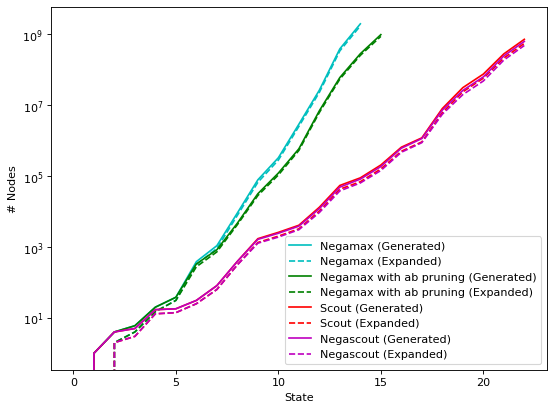
\includegraphics[scale=0.5]{figura1.png}
  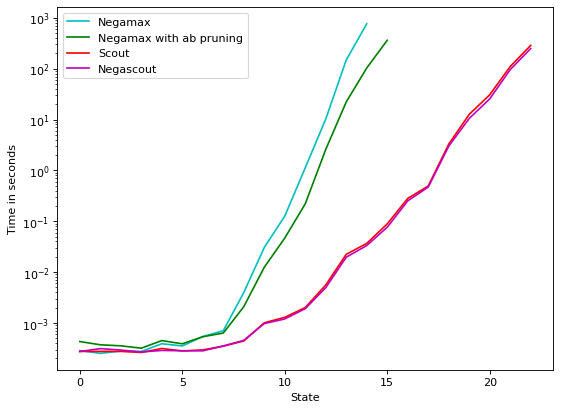
\includegraphics[scale=0.5]{figura2.png} \\ 
  \small{\textit{Figuras 1 y 2. A la izquierda, nodos generados y expandidos 
  por cada algoritmo en cada estado de la PV sin usar TT. A a la derecha, tiempo de 
  ejecuci\'on por cada algoritmo en cada estado de la PV sin usar TT.}}\\
  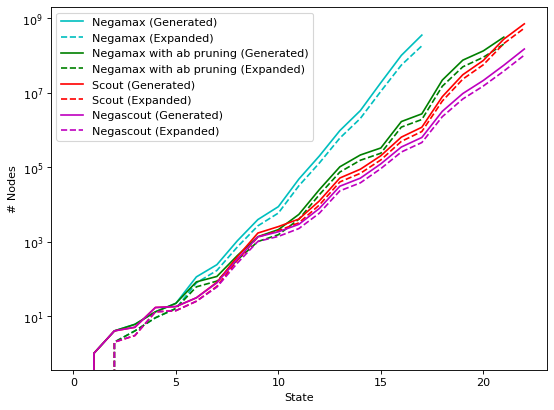
\includegraphics[scale=0.5]{figura5.png}
  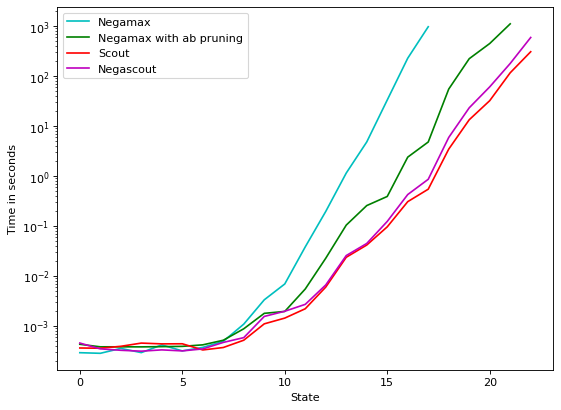
\includegraphics[scale=0.5]{figura6.png}
  \\
  \small{\textit{Figuras 3 y 4. A la izquierda, nodos generados y expandidos por cada 
  algoritmo en cada estado de la PV usando TT. A la derecha, tiempo de ejecuci\'on por 
  cada algoritmo en cada estado de la PV usando TT}}
\end{figure*}


\section*{Extra: game.cpp}
  Adicionalmente, cre\'o este archivo para poder jugar othello 6x6 en contra de la IA. Para 
  compilarlo se debe ejecutar \verb|make game| en la raiz del repositorio del proyecto. Una vez 
  compilado, se crear\'a un ejecutable \verb|game.out| dentro del directorio \verb|bin/| cuya 
  sintaxis es 

  \begin{center}
    \verb|game.out DEPTH BLACKS|
  \end{center}

  \noindent
  donde \verb|DEPTH| es la profundidad m\'axima para la b\'usqueda en el \'arbol de juego, y 
  \verb|BLACKS| indica si el jugador ser\'a las negras (\verb|1|) o las blancas (\verb|0|). Se 
  usa siempre \verb|scout| sin tabla de transposici\'on. Cada jugada debe indicarse 
  seg\'un la fila (enumeradas del 1 al 6) y la columnas (identificadas de la a a la f), por ejemplo, 
  \verb|3c|. En caso de que se deba pasar, se escribe \verb|P|.

\section*{Conclusiones}
  \begin{itemize}
    \item Negamax es el m\'as ineficiente de los algoritmos probados.
    \item La poda alpha-beta ayuda bastante al algoritmo negamax.
    \item Los algoritmos scout y negascout tienen un rendimiento muy similar, por lo que la poda 
    alpha-beta no es muy efectiva en scout.
    \item El n\'umero de nodos expandidos no se aleja mucho del n\'umero de nodos generados.
    \item Las tablas de transposici\'on mejoran bastante el rendimiento de negamax, m\'as aun si 
    utiliza poda alpha-beta.
    \item Las tablas de transposici\'on no mejoran a los algoritmos scout y negascout, incluso 
    puede hacerlos m\'as ineficientes en tiempo, adem\'as de que obviamente es mucho m\'as ineficiente 
    en memoria debido a la gran cantidad de estados que debe almacenar.
    \item Para implementar un juego con IA, las mejores opciones son scout y negascout sin tablas 
    de transposici\'on.
  \end{itemize}


\end{document}